\documentclass[10pt,twocolumn,letterpaper]{article}

\usepackage{cvpr}
\usepackage{times}
\usepackage{epsfig}
\usepackage{graphicx}
\usepackage{amsmath}
\usepackage{amssymb}

% Include other packages here, before hyperref.
\usepackage{booktabs}
\usepackage{caption}
\usepackage{subcaption}
\usepackage{array}
\usepackage{tabularx}
\usepackage{bm}
\usepackage{multirow}
\usepackage{float}
\usepackage[utf8x]{inputenc}
\usepackage{mathtools}
\DeclarePairedDelimiter{\paren}{\lparen}{\rparen}
\DeclarePairedDelimiter{\bracket}{[}{]}
\DeclarePairedDelimiter{\ang}{\langle}{\rangle}
\DeclarePairedDelimiter{\abs}{\lvert}{\rvert}
\DeclarePairedDelimiter{\set}{\{}{\}}
\DeclarePairedDelimiter{\norm}{\|}{\|}
\DeclareMathOperator{\dom}{dom}
% The above let you do things like:
% Let $A = \set{1,2,\ldots,n}$...

\newtheorem{thm}{Theorem}
\newtheorem{lem}[thm]{Lemma}
\newtheorem{prop}[thm]{Proposition}
\newtheorem{cor}[thm]{Corollary}
\newtheorem{defn}{Definition}[section]
\newtheorem{conj}[thm]{Conjecture}

\newcommand{\alg}[1]{\begin{algorithm}\begin{algorithmic}[0]#1\end{algorithmic}\end{algorithm}}
\newcommand{\eqn}[1]{\begin{equation*}#1\end{equation*}}
\newcommand{\eqnsplit}[1]{\begin{equation}\begin{split}
#1
\end{split}\end{equation}}
\newcommand{\txt}[1]{\textrm{#1}}
\newcommand{\s}[1]{\section{#1}}
\newcommand{\sbs}[1]{\subsection{#1}}

\newcommand{\id}{\mathrm{id}}
\newcommand{\divs}{\mid}
\newcommand{\tdivs}{\,\Big\vert\,}
\newcommand{\ndivs}{\nmid}

\newcommand{\mset}[2]{\set{\, #1 \mid #2 \,}}
\newcommand{\msset}[2]{\left\{\, #1 \;\middle\vert\; #2 \,\right\}}
\newcommand{\smat}[1]{\paren*{\begin{smallmatrix} #1 \end{smallmatrix}}}
\newcommand{\ord}[1]{\left| #1 \right|}
% Blackboard bold.
\newcommand{\N}{\mathbb{N}}
\newcommand{\Z}{\mathbb{Z}}
\newcommand{\Q}{\mathbb{Q}}
\newcommand{\R}{\mathbb{R}}
\newcommand{\F}{\mathbb{F}}
\newcommand{\E}{\mathbb{E}}

\newcommand{\X}{\mathcal{X}}

% Other
\newcommand{\del}{\partial}
\newcommand{\Real}{\text{Re}}
\newcommand{\Imag}{\text{Im}}
\newcommand{\res}{\text{res}}



% If you comment hyperref and then uncomment it, you should delete
% egpaper.aux before re-running latex.  (Or just hit 'q' on the first latex
% run, let it finish, and you should be clear).
\usepackage[pagebackref=true,breaklinks=true,letterpaper=true,colorlinks,bookmarks=false]{hyperref}

% \cvprfinalcopy % *** Uncomment this line for the final submission

\def\cvprPaperID{****} % *** Enter the CVPR Paper ID here
\def\httilde{\mbox{\tt\raisebox{-.5ex}{\symbol{126}}}}

\graphicspath{{"G:/Shared drives/Stanford Computational Imaging/Projects/single_spad_depth/figures/"}{"/Volumes/GoogleDrive/Shared drives/Stanford Computational Imaging/Projects/single_spad_depth/figures/"}{}}
% Pages are numbered in submission mode, and unnumbered in camera-ready
\ifcvprfinal\pagestyle{empty}\fi
\begin{document}

%%%%%%%%% TITLE
\title{Optimizing Monocular Depth Estimation with Global Depth Histogram Matching using a Single SPAD}

\author{First Author\\
Institution1\\
Institution1 address\\
{\tt\small firstauthor@i1.org}
% For a paper whose authors are all at the same institution,
% omit the following lines up until the closing ``}''.
% Additional authors and addresses can be added with ``\and'',
% just like the second author.
% To save space, use either the email address or home page, not both
\and
Second Author\\
Institution2\\
First line of institution2 address\\
{\tt\small secondauthor@i2.org}
}

\maketitle
%\thispagestyle{empty}

%%%%%%%%% ABSTRACT
\begin{abstract}
abstract
\end{abstract}

%%%%%%%%% BODY TEXT

\section{Introduction}
\label{sec:intro}
%
\subsection{Context}
Estimating depth from images is an important imaging problem, as dense depth
maps are useful precursors for high-level scene understanding tasks like
segmentation and pose estimation (cite cite cite) and mid-level perception (of
which depth estimation is an important part) has been shown to be very useful
for e.g. training robots to navigate their environments. While traditional approaches to depth
estimation use multiple cameras or structure-from-motion, convolutional neural
networks have also demonstrated reasonable performance on the so-called
monocular depth estimation task, where the network is trained to produce a dense
depth map given only a single RGB image of the scene.
\subsection{Problem Statement}
While deep monocular depth estimators have demonstrated strong performance (cite
cite) and even some generalizability across scene types, the task they are solving is fundamentally
underconstrained due to \textit{inherent scale ambiguity}, i.e. the unresolvable
tradeoff between size and distance in monocular images. This ambiguity could be
resolved by adding an additional camera and calculating a disparity map, but
this method still fails on textureless regions and areas with lots of
occlusions. Other approaches use FMCW or time-of-flight LiDAR technologies,
but these approaches are currently expensive and bulky. 
\subsection{Proposed approach}
In this paper, we show that by augmenting the RGB image with a histogram of
depth information, we can achieve substantially improved performance
(and generalizability) over state-of-the-art monocular depth
estimators. By performing an exact, weighted histogram matching on the output
depth map of the depth estimator, we can match the depth histogram of the scene
to the depth histogram of our estimate. Such a histogram can be captured
relatively inexpensively using only a single pixel single-photon avalanche diode
(SPAD) and pulsed laser illumination diffused over the field of view.
\subsection{Impact}
Our method is a lightweight postprocessing step that substantially improves
the quality of depth maps produced by monocular depth estimators. It can be
applied to any method to improve the accuracy instantly. (Our method also
helps neural-network-based methods generalize across scene types easily.)
\subsection{Limitations}
Our method is not without limitations, however. It still requires a laser and
single-pixel detector, and as such, is sensitive to ambient photons. Our method,
which is a fundamentally a variant of histogram matching, is, like histogram
matching, unable to transpose the values of pixels (i.e. if pixel $a$ is farther
than pixel $b$ in the input, it will be farther than pixel $b$ in the output).
In other words, our method is not able to resolve ordinal depth errors
(errors where an object is wrongly placed closer or farther
relative to another object). Finally, our method is non-differentiable, and is
therefore unsuitable for end-to-end optimization of multi-part networks.

\begin{itemize}
	\item We introduce the idea of augmenting an RGB camera with a single-pixel
    SPAD to address scale ambiguity error in monocular depth estimators.	
  \item We analyze our approach on indoor scenes using the NYU Depth v2 dataset.
    We demonstrate that our approach is able to resolve scale ambiguity while
    being fast and easy to implement.
  \item (Potentially) We investigate the ability of our method to 
    help generalization of monocular depth estimators across scene types. 
    We (hopefully) demonstrate that our method allows monocular depth
    estimators to perform well even on completely different scene types.
	\item We build a hardware prototype and evaluate the efficacy of our
    approach on real-world data. 
\end{itemize}




\section{Related Work}
\label{sec:related}
% \paragraph{Depth Imaging}
% Include in intro, don't necessarily need it here.
% Conventional approaches to estimating depth from images include stereo-based
% approaches 
% \begin{itemize}
% 	\item stereo and multiview
% 	\item structured illumination and random patterns (kinect, etc.), active stereo
% 	\item time of flight (continuous wave and pulsed)
% 	\item what we do: like pulsed but much simpler setup; no scanning, no spad array, ...
% \end{itemize}


%%%%%%%%%%%%%%%%%%%%%%%%%%%%%%%%%%%%%%%%%%%%%%%%%%%%%%%%%%%%%%%%%%%%%%%%%%%%%%%%%%%%%%%%%%%%%%%%%
\paragraph{Monocular Depth Estimation}
%
Estimating a depth map from a single RGB image has been approached using Markov Random Fields~\cite{Saxena2006}, geometric approaches~\cite{Hoiem2005}, and non-parametric, SIFT-based methods~\cite{Karsch2014}. More recently, deep neural networks have been applied to this problem. For example, Eigen et al.~\cite{Eigen2014} use a multi-scale neural network to
predict depth maps, Godard et al.~\cite{Godard2017} use an unsupervised approach that trains a network using stereo pairs, and Fu et al.~\cite{Fu2018} combine a logarithmic depth discretization scheme with an ordinal regression loss function. Various experiments using different types of encoder networks (\eg ResNet, DenseNet)~\cite{Alhashim2018,Laina2016} have also been employed with some success, as have approaches mixing deep learning with conditional random fields~\cite{Xu2017}, and attention-based approaches~\cite{Hao2018,Xu2018}. Recently, Lasinger et al.~\cite{Lasinger:2019} improved the robustness of monocular depth estimation using cross-dataset transfer.

Despite achieving remarkable success on estimating ordinal depth from a single image, none of these methods are able to resolve inherent scale ambiguity in a principled manner. We introduce a new approach that leverages existing monocular depth estimation networks and disambiguates the output using depth histogram-like measurements obtained from a single, diffused SPAD. Other approaches to disambiguating monocular depth estimation use optimized freeform lenses~\cite{Chang:2019:DeepOptics3D,Wu:2019} or dual-pixel sensors~\cite{Garg:2019}, but these approaches require custom lenses or sensors and specialized image reconstruction methods. In contrast, our approach is potentially compatible with existing camera systems (\eg deployed on current cell phones) and our algorithms could be used in tandem with existing camera ISPs.

%%%%%%%%%%%%%%%%%%%%%%%%%%%%%%%%%%%%%%%%%%%%%%%%%%%%%%%%%%%%%%%%%%%%%%%%%%%%%%%%%%%%%%%%%%%%%%%%%
\paragraph{Depth Imaging and Sensor Fusion with SPADs}
%
Emerging single-photon LiDAR systems use single-photon avalanche diodes (SPADs)
to record the time of flight of individual photons. SPAD detectors can be
fabricated using standard CMOS processes, but the required picosecond-accurate
time-stamping electronics are challenging to miniaturize and fabricate at low
cost. For this reason, many single-photon 3D imaging approaches use a single
SPAD combined with a raster scanning
mechanism~\cite{Kirmani:2014,Lamb2010,Li:2019,pawlikowska2017single,gupta2019photonflooded}.
Unfortunately, this makes it challenging to scan dynamic scenes at high
resolution and scanners can also be expensive, difficult to calibrate, and prone
to mechanical failure. To reduce the scanning complexity to one dimension, 1D
SPAD arrays have been
developed~\cite{burri2017linospad,burri2016linospad,OToole2017}, and 2D SPAD
arrays are also an active area of
research~\cite{Niclass2005,Stoppa2007,Veerappan2011,Zhang2018}. Yet,
single-pixel SPADs remain the only viable option for low-cost consumer devices
today.


The proposed method uses a single-pixel SPAD and pulsed light source that are
diffused across the entire scene instead of aimed at a single point, as with
proximity sensors. This unique configuration captures a measurement that closely
resembles the depth histogram of the scene. Our sensor fusion algorithm achieves
reliable absolute depth estimation by combining the SPAD measurement with the
output of a monocular depth estimator using a histogram matching technique.
While other recent work also explored RGB-SPAD sensor fusion~\cite{Lindell2018},
the RGB image was primarily used to guide the denoising and upsampling of
measurements from a SPAD array.

 
%Previous work (see \cite{Horaud2016} for a survey) has been able to use
%single-pixel SPADs \cite{Lamb2010} and also 1D LinoSPADs in tandem with various
%scanning or DMD devices to capture 3D volumes of photon arrivals that can be
%used to reconstruct depth. Lindell et. al. \cite{Lindell2018} use a LinoSPAD
%and epipolar scanline and fuse the SPAD data with an RGB image to produce
%high-quality depth.  Our approach uses a single pixel SPAD but does not require
%any scanning or DMD mechanism.


%A parallel approach called 3D flash LiDAR uses a laser with an optical diffuser
%as the illumination source and a 2D array of SPADs to capture the 3D volume
%\cite{Stoppa2007, Niclass2005}. Such arrays are capable of reconstructing high
%quality depth but remain relatively low resolution. Other arrays are able to
%achieve higher resolution, but suffer from low fill factor \cite{Veerappan2011} or
%sacrifice per-pixel TDC \cite{Zhang2018}.

% \begin{itemize}
%   \item Scanned single-pixel and 1D arrays, but scanning is hard
%   \item high resolution arrays -> challenging to do TDC
%   \item Individual (non-scanning) SPADs already exist in e.g. iPhoneX, but use
%     is limited to proximity sensors.
%   \item What we do: No array (easier), no scanning (easier), much cheaper,
%     combined with RGB camera to do high-resolution depth imaging, a more complex
%     task.
% \end{itemize}

%%%%%%%%%%%%%%%%%%%%%%%%%%%%%%%%%%%%%%%%%%%%%%%%%%%%%%%%%%%%%%%%%%%%%%%%%%%%%%%%%%%%%%%%%%%%%%%%%
% \paragraph{Deep Sensor Fusion}
% Maybe mention in previous section? 
% global hints for super-resolution, colorization, depth estimation 
%
% \begin{itemize}
	% \item colorization
	% \item david's 2018 paper for depth estimation and denoising (see david's 2019 sig paper for related work)
	% \item what we do: slightly different application
% \end{itemize}

%%%%%%%%%%%%%%%%%%%%%%%%%%%%%%%%%%%%%%%%%%%%%%%%%%%%%%%%%%%%%%%%%%%%%%%%%%%%%%%%%%%%%%%%%%%%%%%%%
\paragraph{Histogram Matching and Global Hints}
%
Histogram matching is a well-known image processing technique for adjusting an
image so that its histogram matches some pre-specified histogram (often derived
from another image)~\cite{gonzales1977gray,Gonzalez2008}. Nikolova et
al.~\cite{Nikolova2013} use optimization to recover a strict ordering of the
image pixels, yielding an exact histogram match. Morovic et
al.~\cite{Morovic2002} provide an efficient and precise method for fast
histogram matching which supports weighted pixel values. In the image
reconstruction space, Swoboda and Schn\"orr~\cite{Swoboda2013} use a histogram
to form an image prior based on the Wasserstein distance for image denoising and
inpainting. Rother et al.~\cite{Rother2006} use a histogram prior to create an
energy function that penalizes foreground segmentations with dissimilar
histograms. In a slightly different application area, Zhang et
al.~\cite{Zhang2017} train a neural network to produce realistically colorized
images given only a black-and-white image and a histogram of global color
information.


In our procedure, the diffused SPAD measurements closely resemble a histogram of
the depth map where the histogram values are weighted by spatially varying scene
reflectances and inverse-square falloff effects. We therefore adapt the
algorithm in Morovic et al.~\cite{Morovic2002} in order to accommodate general
per-pixel weights during histogram matching.


% \textcolor{red}{Our method is essentially a modified form of the algorithm in \cite{Morovic2002}, modified for our particular use case. Also worth noting is the fact that most algorithms compute histograms from existing images, whereas our method mesaures the depth histogram indirectly using photon arrivals.} Note: this paragraph needs more work. We can say something like ``Inspired by Morovic et al., we do something'' but then we also need to highlight how our method is different. Perhaps concisely summarize how you adapt it for our SPAD model.
%
% \begin{itemize}
%   \item Exact histogram matching paper used in this work
%   \item Wasserstein-based optimization techniques for
%     histogram-based regularization
% \end{itemize}




\section{Method}
\label{sec:method}
In this section, we describe the measurement model for a single-pixel
time-of-flight lidar sensor under diffuse, pulsed laser illumination. 
\subsection{Measurement Model}
Consider a laser which emits a pulse at time $t = 0$ with time-varying intensity
$g(t)$ uniformly illuminating some 3D scene. We parameterize the geometry of the
scene as a height map $z(x, y)$.
Neglecting albedo and falloff effects, an ideal detector counting photon events
from a location $(x,y)$ in the time interval $(n\Delta t, (n+1) \Delta t)$ would record

\begin{equation}
  \lambda_{x,y}[n] = \int_{n\Delta t}^{(n+1) \Delta t} (f * g)\paren*{t - 2z(x,y)/c} dt \label{single_loc_spad} 
\end{equation}  

where $c$ is the speed of light, and $f$ is a function that models the temporal uncertainty in the
detector. Single-photon avalanche diodes (SPADs) are highly sensitive
photodetectors which are able to record single photon events with high temporal
<<<<<<< HEAD
precision \cite{Stuff}. Since the detection of each photon can be described with
a Bernoulli random variable,
=======
precision \cite{Stuff}. Since the event corresponding to the detection of a
photon can be described with a Bernoulli random variable,
>>>>>>> ac23c73116b7fdd108ca4951a414a00ea9b25df3
the total number of accumulated photons in this time interval follows a Poisson
distribution according to

\begin{equation}
  h[n] \sim \mathcal{P}\paren*{\sum_{x,y}\alpha_{x,y}\eta \lambda_{x,y}[n] + b} \label{global_hints}
\end{equation}

where $\alpha_{x,y} = r_{x,y}/z(x,y)^2$ captures the attenuation of the
photon counts due to the reflectance $r(x,y)$ of the scene and due to the
inverse square falloff $1/z(x,y)^2$.
In addition, $\eta$ is the detection probability of a photon
triggering a SPAD event, and $b = \eta a + d$ is the average number of background detections resulting
from ambient photons $a$
and erroneous ``dark count'' events $d$ resulting from noise within the SPAD.
<<<<<<< HEAD
\newpage
\begin{table*}[htbp]
  \begin{center}
    \begin{tabularx}{\linewidth}{*{2}{X}}
      \includegraphics[width=\textwidth/2-5pt]{sections/figures/spad_example/rgb.png} &
      \includegraphics[width=\textwidth/2-5pt]{sections/figures/spad_example/rawdepth.png} \\
      \includegraphics[width=\textwidth/2-5pt]{sections/figures/spad_example/depth_hist.png} &
      \includegraphics[width=\textwidth/2-5pt]{sections/figures/spad_example/spad_hist.png} \\
    \end{tabularx}
  \end{center}
  \caption{Sample Image. Top Left is the RGB image. Top Right is ground truth
    depth. Bottom Left is Raw ground truth depth histogram. Bottom Right is
    simulated SPAD measurements. Notice how closer depths are magnified and far
    depths are attenuated.}
\end{table*}
=======
% \newpage
% \begin{table*}[htbp]
%   \begin{center}
  %   \begin{tabularx}{\linewidth}{*{2}{X}}
  %     \includegraphics[width=\textwidth/2-5pt]{sections/figures/spad_example/rgb.png} &
  %     \includegraphics[width=\textwidth/2-5pt]{sections/figures/spad_example/rawdepth.png} \\
  %     \includegraphics[width=\textwidth/2-5pt]{sections/figures/spad_example/depth_hist.png} &
  %     \includegraphics[width=\textwidth/2-5pt]{sections/figures/spad_example/spad_hist.png} \\
  %   \end{tabularx}
  % \end{center}
  % \caption{Sample Image. Top Left is the RGB image. Top Right is ground truth
  %   depth. Bottom Left is Raw ground truth depth histogram. Bottom Right is
  %   simulated SPAD measurements. Notice how closer depths are magnified and far
  %   depths are attenuated.}
% \end{table*}
>>>>>>> ac23c73116b7fdd108ca4951a414a00ea9b25df3

\subsection{Monocular depth estimation with global depth hints}
Given a single RGB image $I(x,y)$ and a vector of photon arrivals $h[n]$
described by equation \ref{global_hints}, we seek to
reconstruct the ground truth depth map $z(x,y)$.
<<<<<<< HEAD
Our method has two parts. First, we initialize our estimate of the depth map from the single RGB
image via a monocular depth estimator described below. Second, we refine this depth map using
the captured measurements $h[n]$ via a process we call Differentiable Histogram
Matching (DHM).
Differentiable histogram matching is a tool for post-processing the image to
match the depth map to the statistics we capture from the SPAD.

\paragraph{Initialization via CNN}
Convoluational Neural Networks have become increasingly capable of leveraging
monocular depth cues to produce accurate estimates of depth
from only a single image. We therefore choose to initialize our depth map
estimate $\hat z^{(0)}(x,y)$ using
a CNN. However, any depth estimator reliant on only a single
view will be unable to resolve the inherent scale ambiguity in the scene resulting
from the tradeoff between size of and distance to an object. The next step,
differentiable histogram matching, will resolve this ambiguity using the depth
information present in the SPAD histogram.

\paragraph{SPAD Denoising}
\begin{itemize}
  \item Discuss MLE for SPAD denoising
  \item Write optimization problem for SPAD denoising
  \item Show performance on a few examples 
\end{itemize}
=======
Our method has two parts. First, we \textbf{initialize} our estimate of the depth map from the single RGB
image via a monocular depth estimator described below. Second, we \textbf{refine} this depth map using
the captured measurements $h[n]$ via exact histogram matching. 

\paragraph{Initialization}
The first step in our method is to produce an initial estimate of ground truth
depth. Convolutional Neural Networks have been shown to produce accurate, if poorly-scaled, estimates of depth
from only a single image. We therefore choose to initialize our depth map
estimate $\hat z^{(0)}(x,y)$ using
a CNN. However, any depth estimator reliant on only a single
view may be used for this step. Furthermore, in the larger context of our
algorithm, it is more important that the network predict the correct ordinal
relationships between pixels - that is, to predict the correct relative ordering
of pixels $a$ and $b$, rather than to get all pixels exactly correct.

>>>>>>> ac23c73116b7fdd108ca4951a414a00ea9b25df3
\paragraph{Exact Histogram Matching}
\begin{figure}
  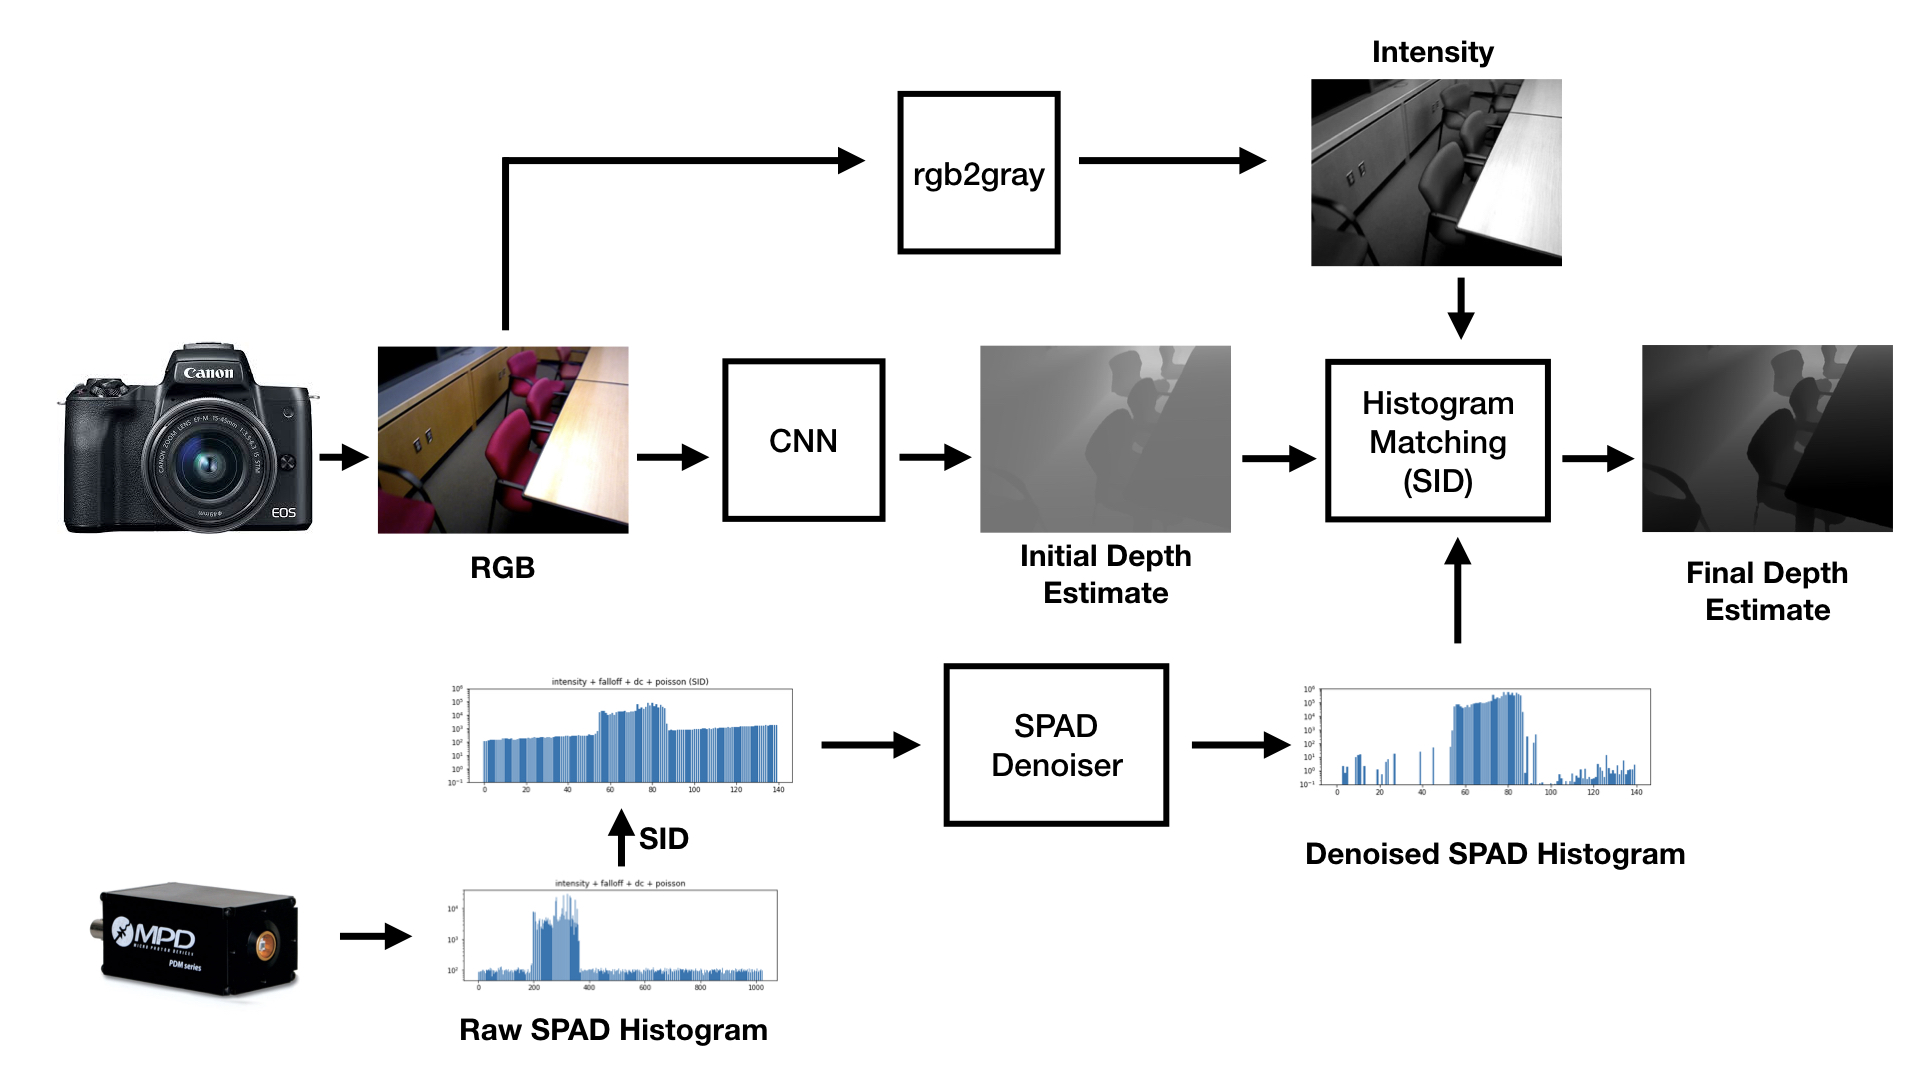
\includegraphics[width=\textwidth/2]{sections/figures/full_pipeline/full_pipeline.jpeg}
  \caption{\textbf{Overview of the full pipeline} We use a CNN to get an initial
<<<<<<< HEAD
  per-pixel depth estimate. We then perform gradient descent to optimize that
  estimate using the SPAD forward model and the dual-Sinkhorn distance
  .}
=======
  per-pixel depth estimate. Then we perform exact histogram matching using
  intensity-weighted pixel values on the corrected SPAD data.}
>>>>>>> ac23c73116b7fdd108ca4951a414a00ea9b25df3
\end{figure}
An image's \textit{histogram} is a pair of vectors $(h, b)$ where $h_i$ is the number of
pixels of the image whose value lies in the range $[b_i, b_i+1)$.
Then, given a source image $S$ with histogram $(h_s, b)$ and a target histogram
$(h_t, b)$, histogram matching generates a new image $M$ such that $h_m \approx
h_t$ and the pixel values in $M$ are in the same relative order as in $S$.
<<<<<<< HEAD


=======
The full details of the exact histogram matching algorithm can be found in
\cite{Morovic2002}.

However, for our purposes, we need to modify our algorithm to accommodate
differing per-pixel weights. We can account for squared depth falloff

\paragraph{SPAD Denoising}
\begin{itemize}
  \item Talk about histogram matching in the ideal case, jump straight to intensity 
  \item Talk about histogram matching in our case, and how it approaches the
    ideal case. Discuss the following corrections 
    \begin{itemize}
      \item Ambient/DC - Use \cite{Xin2019} to justify looking for large edges,
        then the ambient estimate to get rid of the noise floor.
      \item Falloff
    \end{itemize}
  \item Talk about how the histogram matching works with intensity
    considerations applied, briefly.
  \item We don't address jitter or poisson noise.
\end{itemize}
\begin{equation}
  h[n] \sim \mathcal{P}\paren*{\sum_{x,y}\alpha_{x,y}\eta \lambda_{x,y}[n] + b} \label{global_hints}
\end{equation}
Given a SPAD with histogram $h$ according to the above equation, we first
process the SPAD to remove the effects of some of the terms. First, we 
>>>>>>> ac23c73116b7fdd108ca4951a414a00ea9b25df3
\subsection{Implementation Details}
For the Monocular Depth Estimator, we use pretrained versions of the
the Deep Ordinal Regression Network (DORN) \cite{} and the DenseDepth Network.
The exact histogram matching method is as described in \cite{}.




\section{Evaluation and Assessment}
\label{sec:evaluation}
\begin{table*}[!t]
\begin{center}
\begin{tabular}{llrrr|rrr}
\toprule
           &                & $\delta1 \uparrow$ & $\delta2 \uparrow$ & $\delta3 \uparrow$ & $rel \downarrow$ & $rmse \downarrow$ & $log10 \downarrow$ \\
model & hyperparams &                    &                    &                    &                  &                   &                    \\
\midrule
\multirow{6}{*}{dorn} & CNN &              0.846 &              0.954 &              0.983 &            0.120 &             0.501 &              0.053 \\
           & CNN + median rescaling &              0.871 &              0.964 &              0.988 &            0.111 &             0.473 &              0.048 \\
           & CNN + GT histogram matching &              0.906 &              0.972 &              0.990 &            0.095 &             0.419 &              0.040 \\
           & Ours (SBR=10) &              0.903 &              0.970 &              0.989 &            0.091 &             0.422 &              0.040 \\
           & Ours (SBR=50) &              0.906 &              0.971 &              0.990 &            0.089 &             0.410 &              0.039 \\
           & Ours (SBR=100) &              0.906 &              0.971 &              0.990 &            0.090 &             0.408 &              0.039 \\
\cline{1-8}
\multirow{6}{*}{densedepth} & CNN &              0.847 &              0.973 &              0.994 &            0.123 &             0.461 &              0.053 \\
           & CNN + median rescaling &              0.888 &              0.978 &              0.995 &            0.106 &             0.409 &              0.045 \\
           & CNN + GT histogram matching &              0.930 &              0.984 &              0.995 &            0.079 &             0.338 &              0.034 \\
           & Ours (SBR=10) &              0.922 &              0.982 &              0.994 &            0.082 &             0.361 &              0.036 \\
           & Ours (SBR=50) &              0.925 &              0.983 &              0.995 &            0.081 &             0.348 &              0.035 \\
           & Ours (SBR=100) &              0.926 &              0.983 &              0.995 &            0.081 &             0.346 &              0.035 \\
\bottomrule
\end{tabular}

\caption{Quantitative evaluation using NYU Depth v2. Bold indicates best
performance for that metric, while underline indicates second best. The proposed
scheme outperforms DenseDepth and DORN on all metrics, and it closely matches or
even outperforms the median rescaling scheme and histogram matching with the
exact depth map histogram, even though those methods have access to ground
truth.}
\vspace{-2em}
\label{tab:comparison}
\end{center}
\end{table*}

\begin{figure*}[!h]
  % 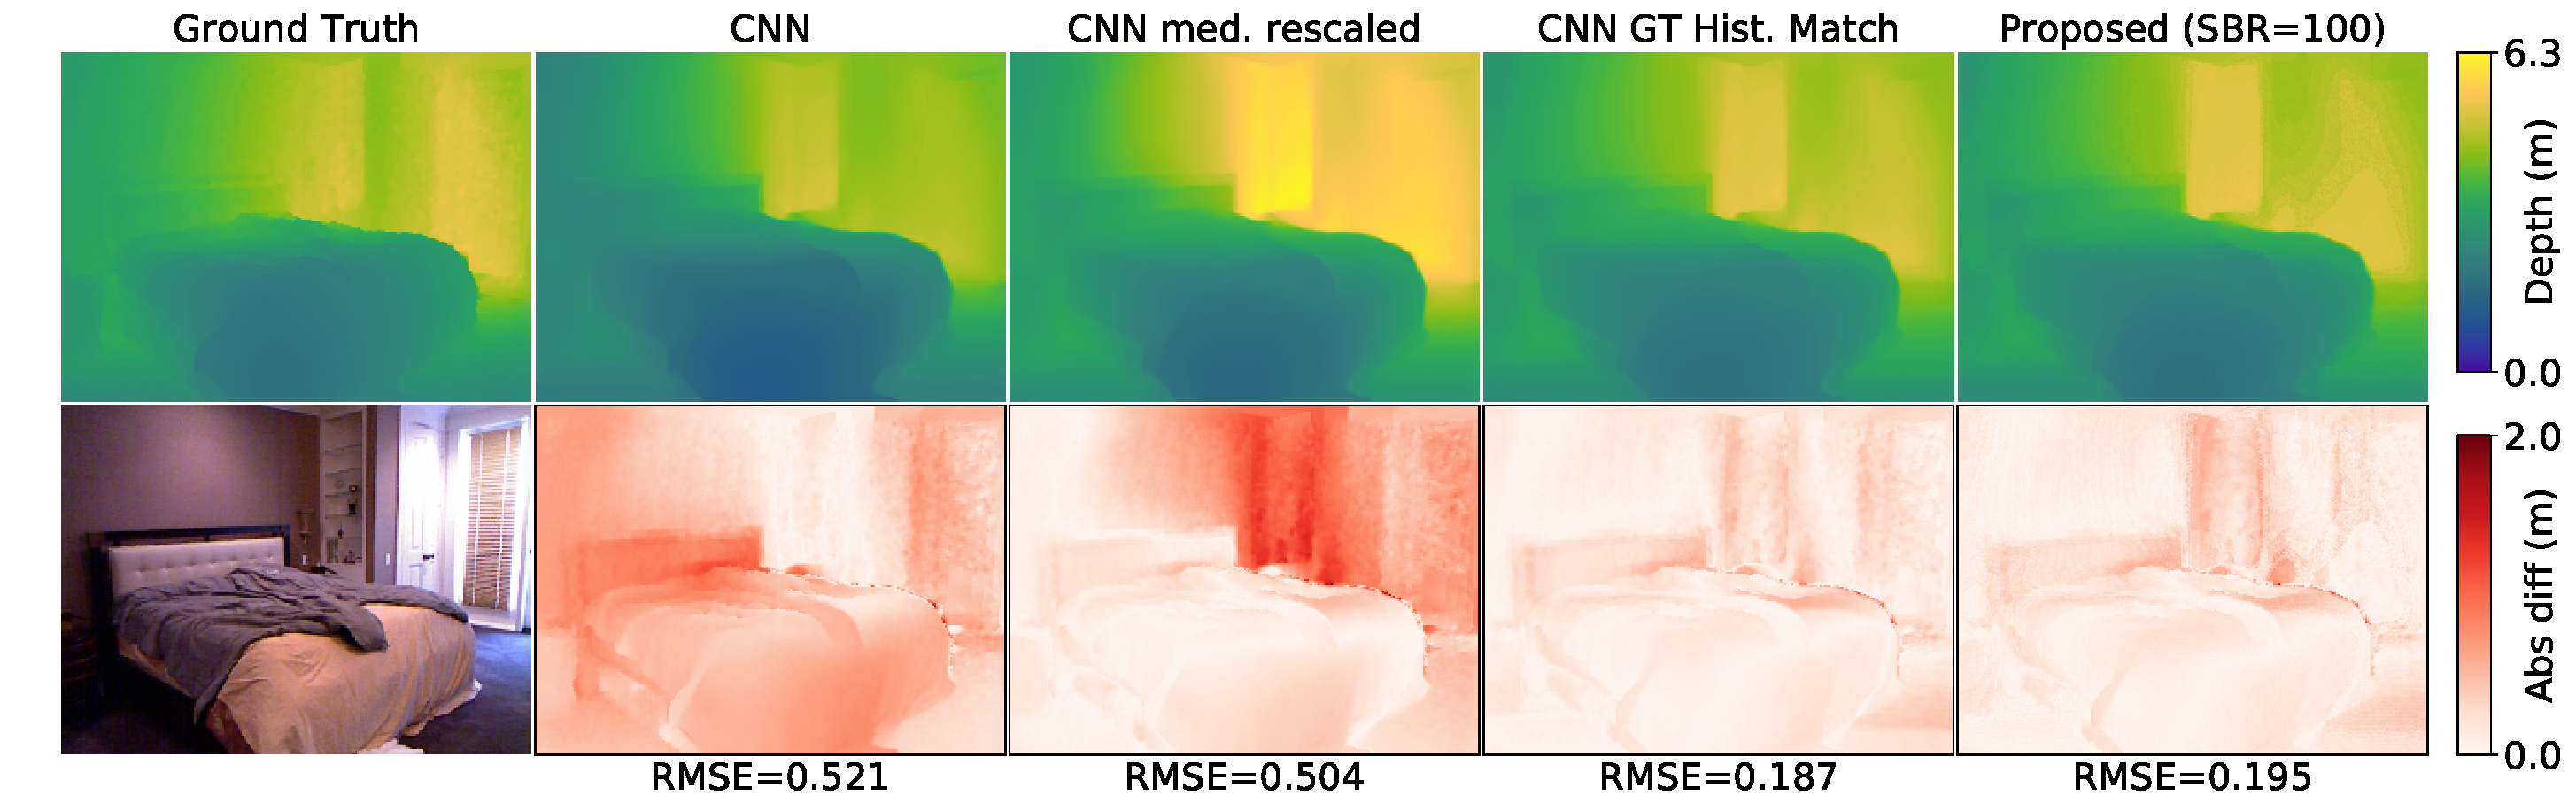
\includegraphics[width=\textwidth]{comparison/densedepth_468_comparison.pdf}
  % 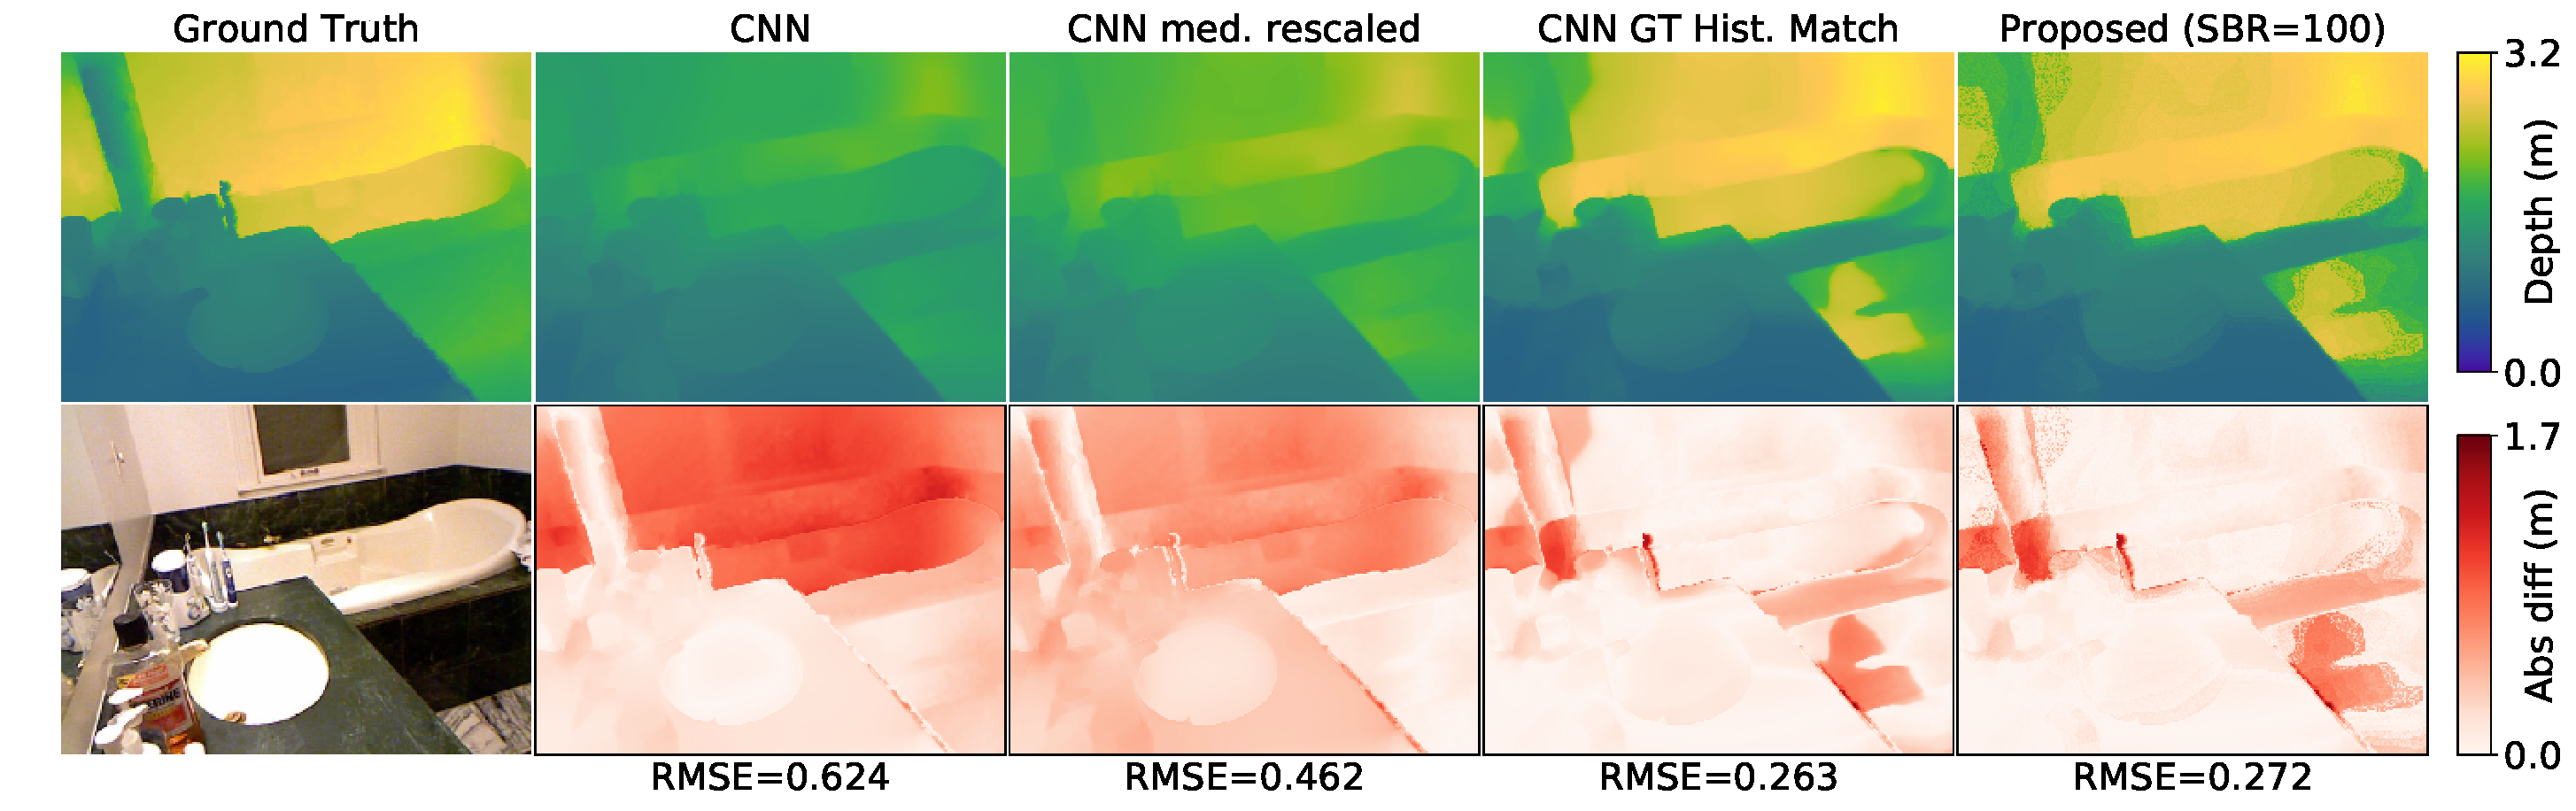
\includegraphics[width=\textwidth]{comparison/densedepth_194_comparison.pdf}
  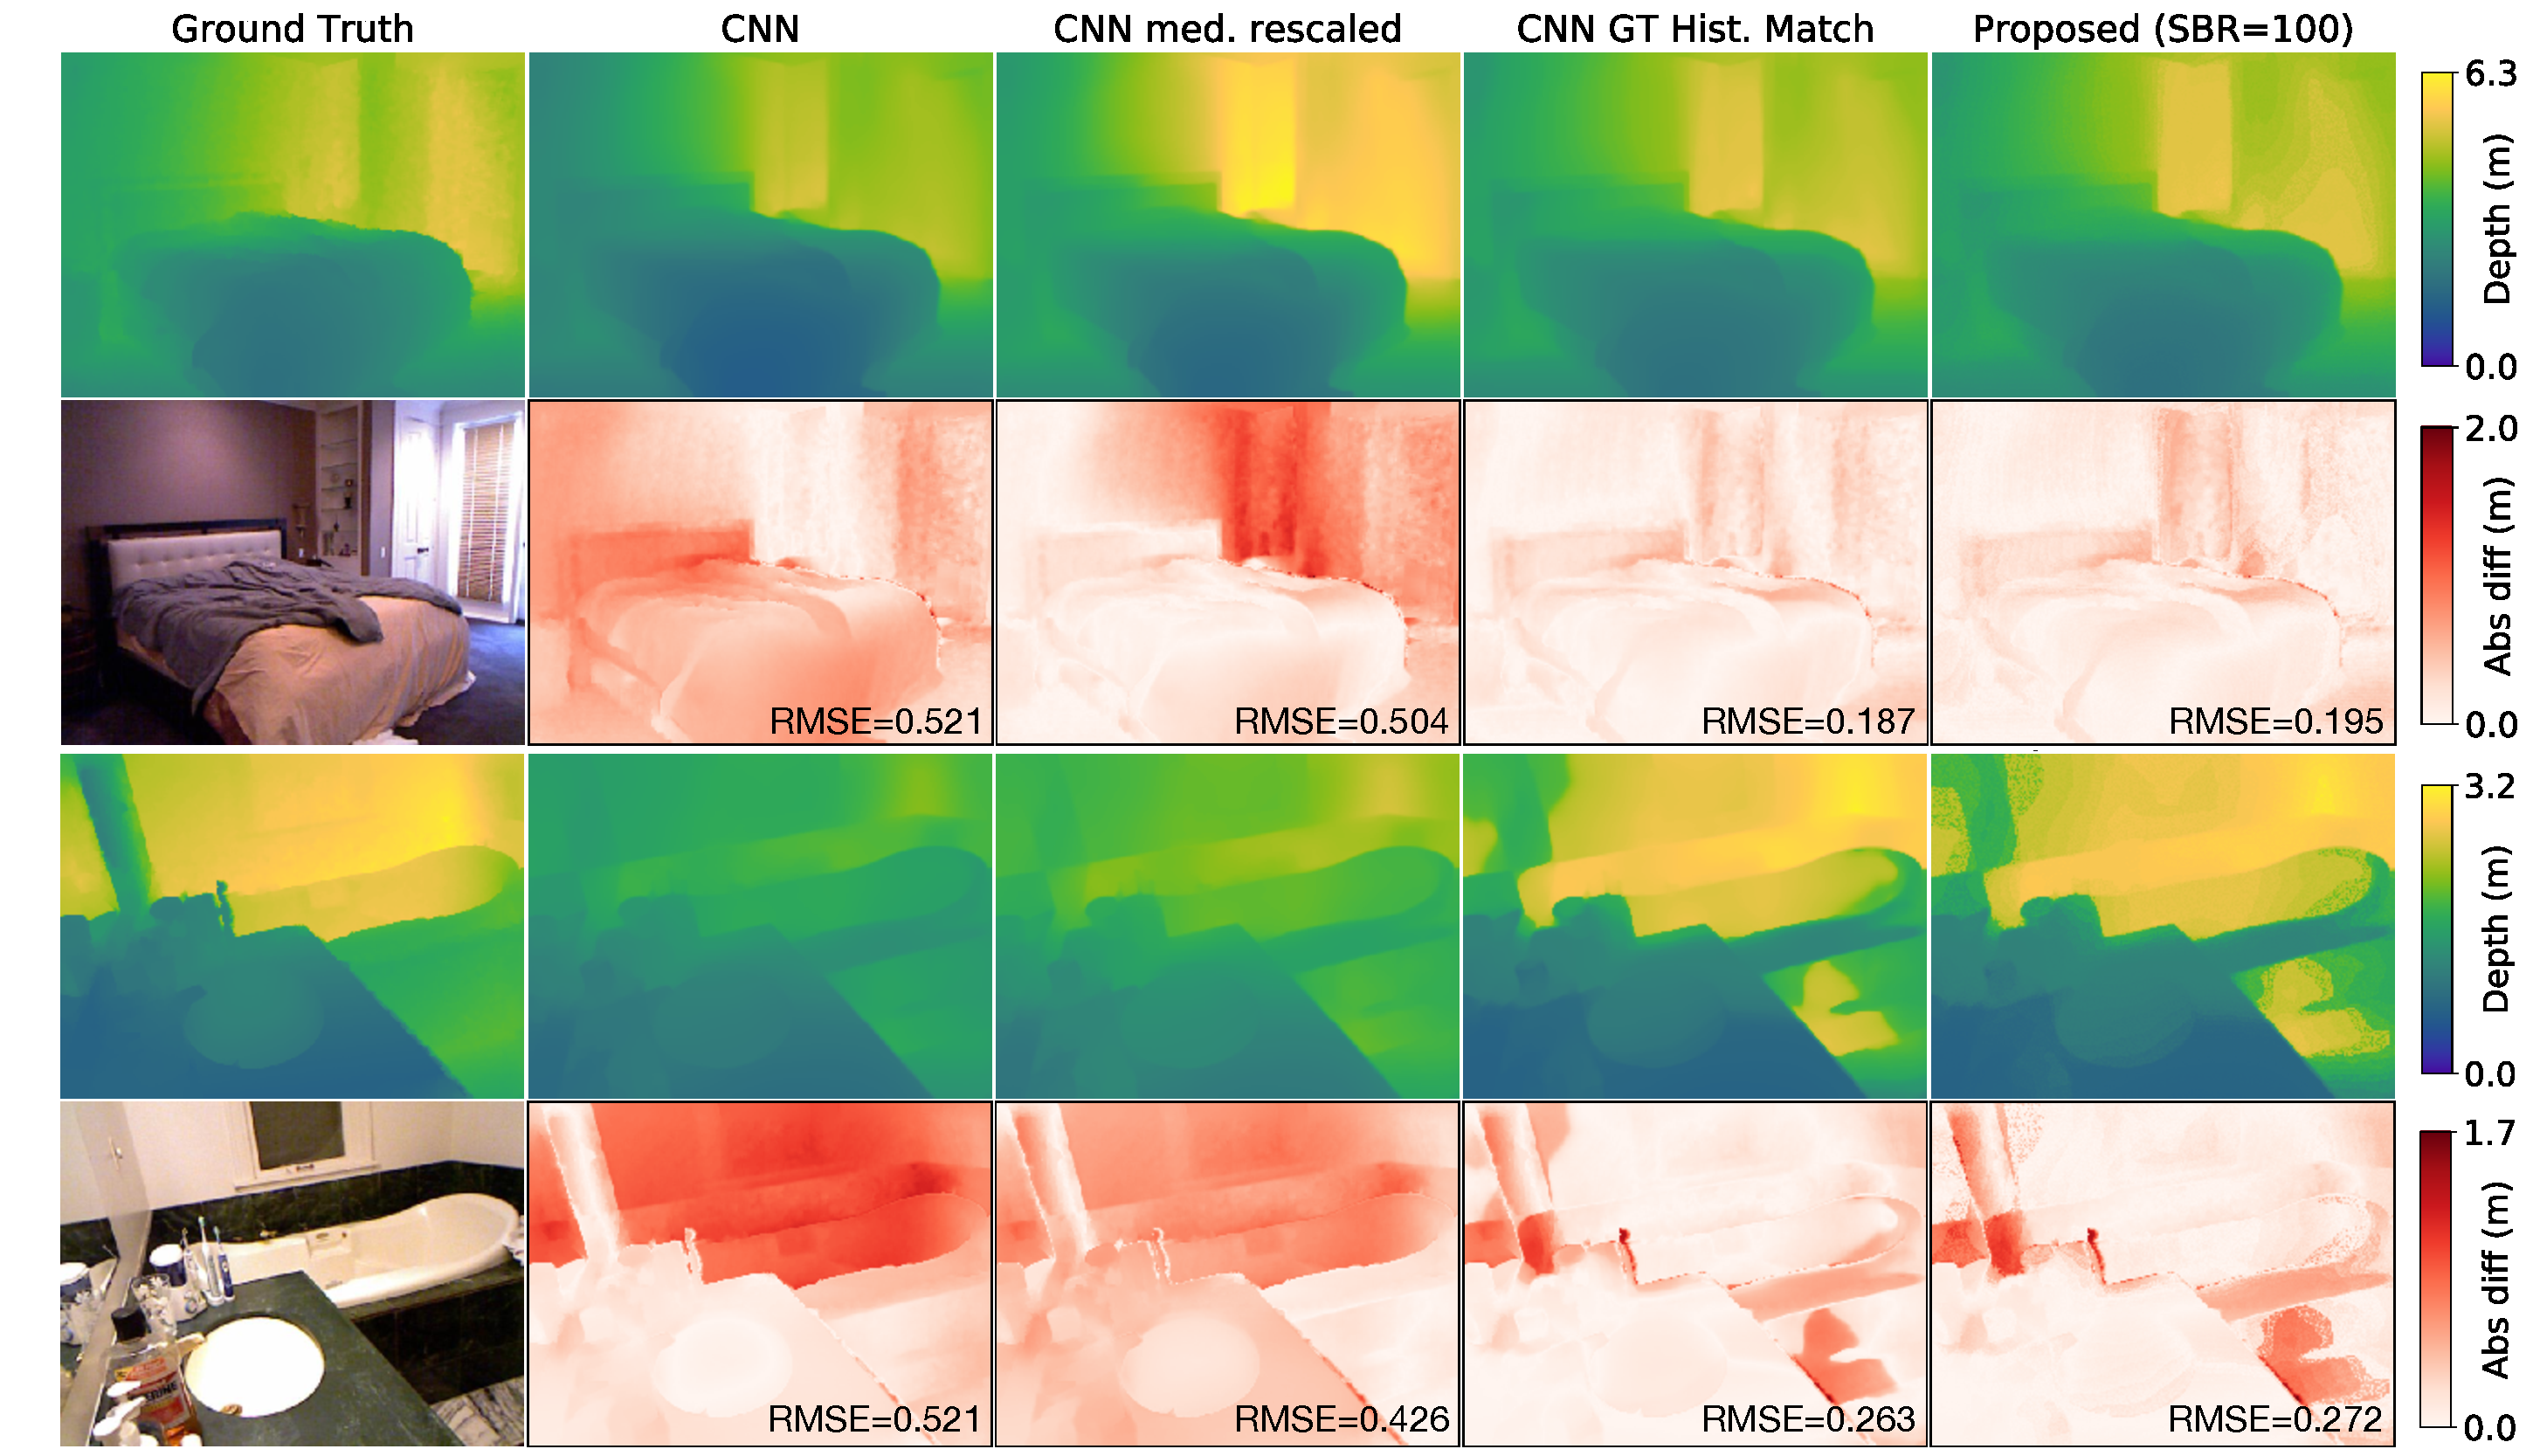
\includegraphics[width=\textwidth]{comparison.pdf}
  %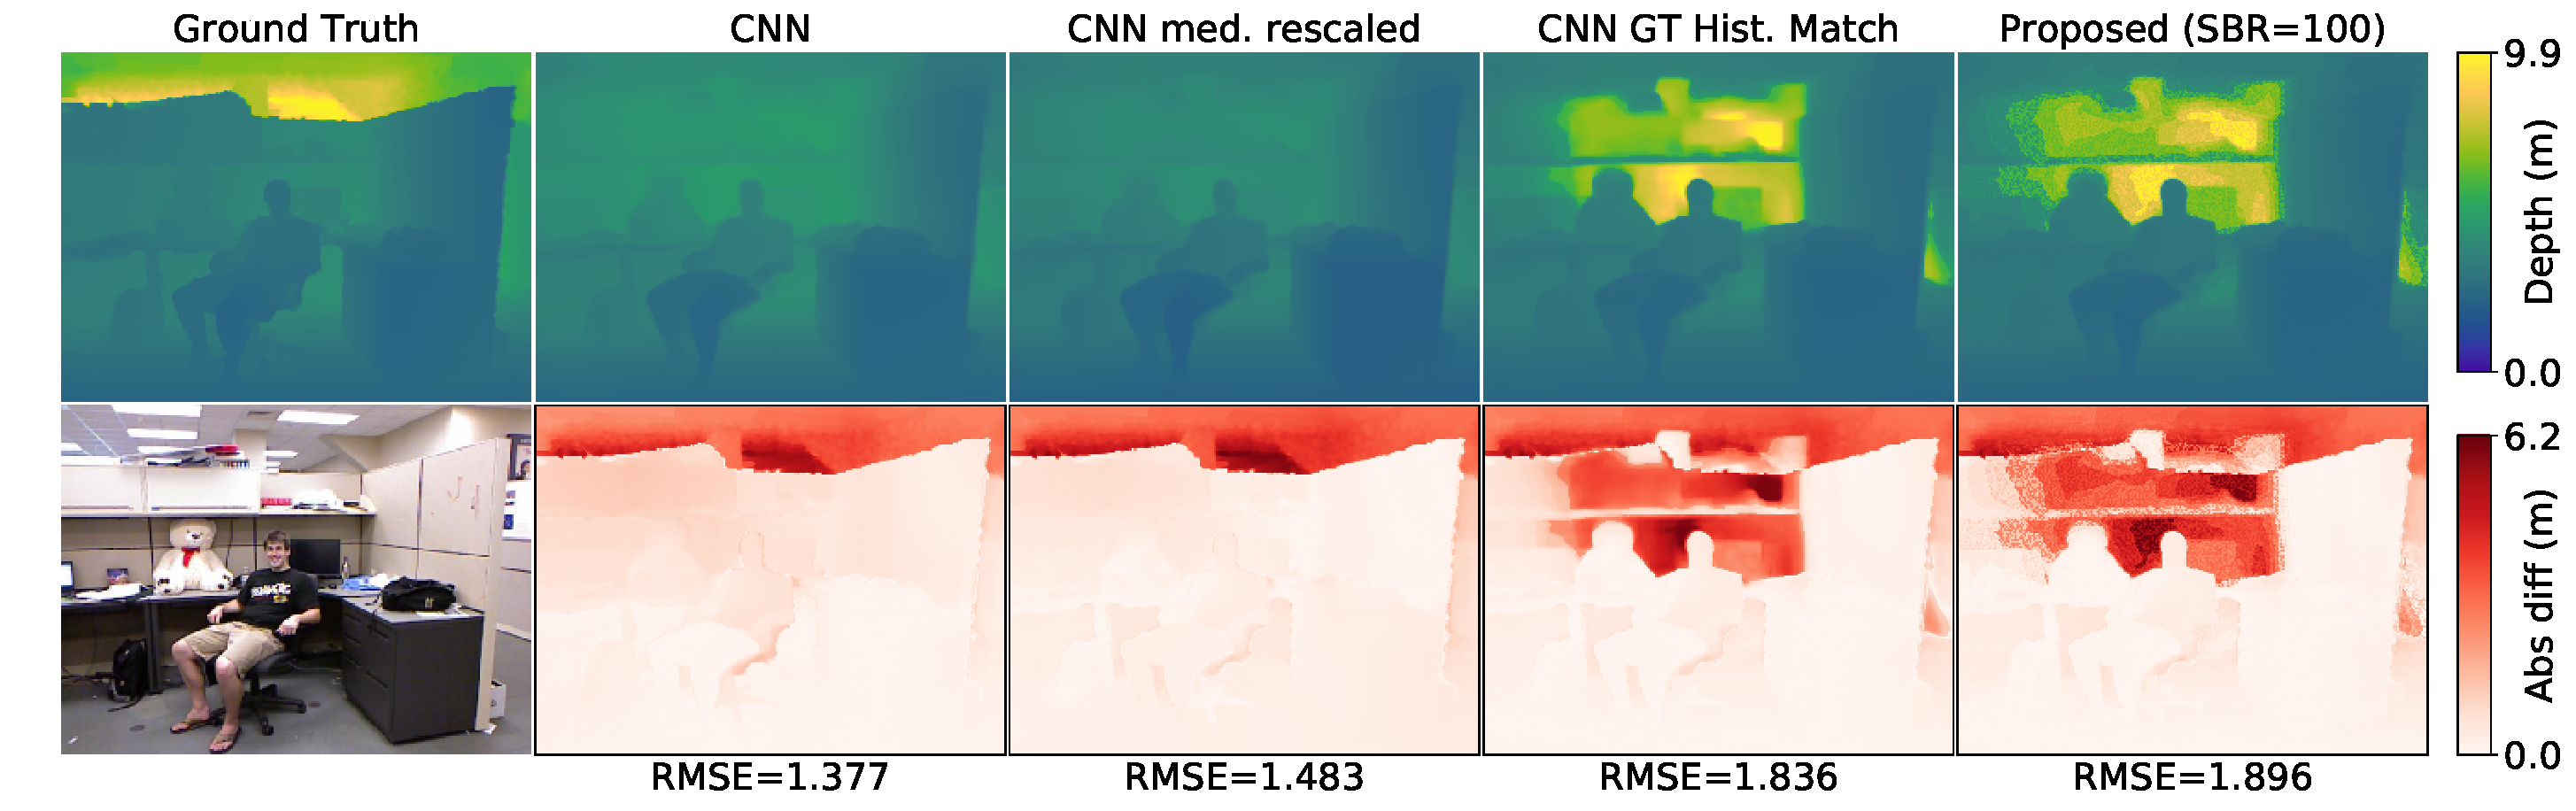
\includegraphics[width=\textwidth]{comparison/densedepth_258_comparison.png}
  \caption{Simulated results from NYU v2 computed with the DenseDepth
  CNN~\cite{Alhashim2018}. The depth maps estimated by the CNN are reasonable,
  but contain systematic error. Oracle access to the ground truth depth maps,
  either through the median depth or the depth histogram, can remove this error
  and correct the depth maps. The proposed method uses measurements from a
  single diffused SPAD and does not rely on ground truth depth, but it achieves
  a quality that closely matches the best-performing oracle.}
	\label{fig:results_simulated}
  \vspace{-1em}
\end{figure*}


%%%%%%%%%%%%%%%%%%%%%%%%%%%%%%%%%%%%%%%%%%%%%%%%%%%%%%%%%%%%%%%%%%%%%%%%%%%%%%%%%%%%%%%%%%%%%%%
\subsection{Implementation Details}

We use the NYU Depth v2 dataset to evaluate our method. This dataset consists of
249~training and 215~testing scenes with RGB-D images captured using a Microsoft
Kinect.

To simulate a SPAD histogram, we take the provided depth map and 
calculate a weighted depth histogram by weighting the pixel contributions to
each depth bin by the luminance of each pixel. To model radiometric falloff, we
multiply each bin by $1/z^2$, and convolve with a modeled system temporal
response, which we approximate as a Gaussian with a full-width at half-maximum of 70~ps. We scale
the histogram by the total number of observed signal photon counts (set to 
$10^6$) and  add a fixed number of background photons $b \in \set{2\times 10^5, 10^5, 2\times
10^4, 10^4}$. The background counts are evenly distributed across all bins to simulate the ambient and dark
count detections, and the different background levels correspond to
signal-to-background ratios (SBR) of $5, 10, 50$ and $100$ respectively. Finally,
each bin is Poisson sampled to produce the final simulated SPAD transient.

%%%%%%%%%%%%%%%%%%%%%%%%%%%%%%%%%%%%%%%%%%%%%%%%%%%%%%%%%%%%%%%%%%%%%%%%%%%%%%%%%%%%%%%%%%%%%%%
\subsection{Simulated Results}

We show an extensive quantitative evaluation in Table~\ref{tab:comparison}.
Here, we evaluate three recent monocular depth estimation CNNs:
DORN~\cite{Fu2018}, DenseDepth~\cite{Alhashim2018}, and
MiDaS~\cite{Lasinger:2019}. To evaluate the quality of DORN and DenseDepth, we
report various standard error metrics~\cite{Eigen2014}. Moreover, we show a simple
post-processing step that rescales their outputs to match the median ground truth
depth~\cite{Alhashim2018}. We also show the results of histogram matching the
output of the CNNs with the ground truth depth map histogram. Note that we do
not report the quality of the direct output of MiDaS as this algorithm does not
output metric depth. However, we do show its output histogram matched with the
ground truth depth map histogram. In all cases, post-processing the estimated
depth maps either with the median depth or depth histogram significantly
improves the absolute depth estimation, often by a large margin compared to the
raw output of the CNNs. Unfortunately, ground truth depth is typically not
accessible so neither of these two post-processing methods are viable in
practical application scenarios.

Instead, our method uses the simulated measurements from a single diffused SPAD
to correct the depth map. In Table~\ref{tab:comparison}, results are shown for several different
signal-to-background ratios (SBRs). We see that the proposed method achieves
high-quality results for correcting the raw depth map estimated by the
respective CNNs for all cases. The quality of the resulting depth maps is almost
as good as that achieved with the oracle ground truth histogram, which can be
interpreted as an approximate upper bound on the performance, despite a
relatively high amount of noise and background signal. These results demonstrate
that the proposed method is agnostic to the specific depth estimation CNN
applied to get the initial depth map and that it generally achieves significant
improvements in the estimated depth maps, clearly surpassing the variation in
performance between depth estimation CNNs.


In Figure~\ref{fig:results_simulated}, we also show qualitative results of our
simulations. For each of these scenes, we show the RGB reference image, the
ground truth depth map, the raw output of the DenseDepth CNN, the result of
rescaling the CNN output with the median ground truth depth, the result of
histogram-matching the CNN output by the ground truth depth map histogram, and
the result achieved by the proposed method for an SBR of 100. Error maps for all
the depth estimation methods are shown. As expected, the CNN outputs depth maps
that look reasonable but that have an average root mean squared error (RMSE) of
about 50--60~cm. Rescaling this depth map to match the median ground truth depth
value slightly improves the quality and histogram-matching with the ground
truth depth histogram shows a large amount of improvement. The quality of the
proposed method is close to using the oracle histogram, despite relying on
noisy SPAD measurements. Additional simulations using DenseDepth and other depth
estimation CNNs for a variety of scenes are shown in the supplement.




\section{Experimental Demonstration}
\label{sec:prototype}

\subsection{Setup}
\begin{figure}[H]
  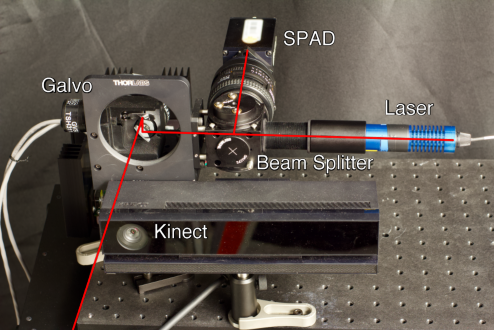
\includegraphics[width=\textwidth/2]{sections/figures/prototype_single_col.png}
  \caption{Prototype scanning setup. The pulsed light from the laser travels
    through a beam splitter before being guided by the galvo to the scene.
    Returning light is measured by the single-pixel SPAD. The RGB camera of a
    Kinect v2 is used to capture the monocular RGB image (the depth camera is
    not used)}
  \label{fig:prototype}
\end{figure}



\section{Discussion}
\label{sec:discussion}
short summary

%%%%%%%%%%%%%%%%%%%%%%%%%%%%%%%%%%%%%%%%%%%%%%%%%%%%%%%%%%%%%%%%%%%%%%%%%%%%%%%%%%%%
\paragraph{Limitations}

\begin{itemize}
	\item laser power vs range tradeoff; may be limited to short--medium range
	\item if the monocular depth estimation fails, so will the histogram matching 
\end{itemize}

%%%%%%%%%%%%%%%%%%%%%%%%%%%%%%%%%%%%%%%%%%%%%%%%%%%%%%%%%%%%%%%%%%%%%%%%%%%%%%%%%%%%
\paragraph{Future Work}


%%%%%%%%%%%%%%%%%%%%%%%%%%%%%%%%%%%%%%%%%%%%%%%%%%%%%%%%%%%%%%%%%%%%%%%%%%%%%%%%%%%%
\paragraph{Conclusions}



{\small
\bibliographystyle{ieee_fullname}
\bibliography{references}
}

\end{document}
